Em relação ao consumo nacional Portugal vem apresentando um crescimento continuo desde 2012, e se consolida em 2016 com um total de  49,3 TWh, um consumo menor apenas 5,6\% do máximo histórico registrado em 2010. Tal crescimento no consumo tem relação direta com o crescimento social e económico do pais, e indica uma tendência para os próximos anos\cite[p.~6]{REN}. 

O gráfico da Figura \ref{fig:ConsumoMax} apresenta a relação dos máximos de consumo e produção registrados desde 2012. Este gráfico torna claro a evolução dos picos de produção sobre os máximos de consumo ao longo dos anos. A relação entre picos de produção e consumo representam uma margem que assegura atendimento da carga mesmo nos dias de maior pico.

\begin{figure}[H]
	\centering
	\captionsetup{width=0.7\textwidth, font=footnotesize, textfont=bf}	
	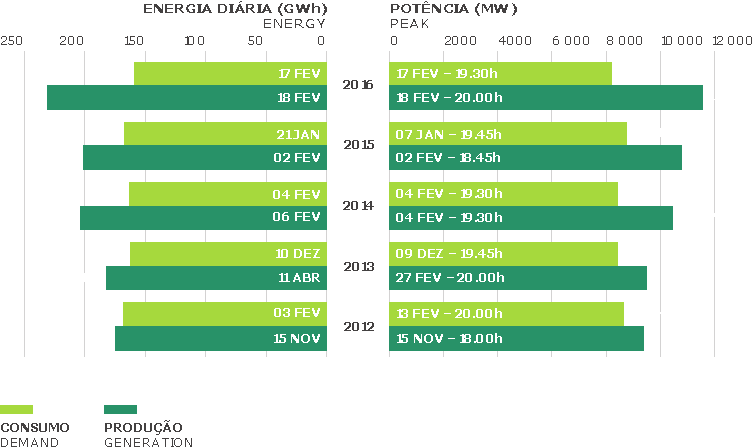
\includegraphics[width=0.7\linewidth]{img/ConsumoEProducaoMaximosAnuais.pdf}
	\caption{Consumo e Produção Máximos Anuais}
	\vspace{-3.5mm}
	\caption*{Fonte: \citeonline{REN}}
	\label{fig:ConsumoMax}
\end{figure}

Em 2016 o dia de maior pico no consumo ocorreu no dia 17 de fevereiro, já em 2015 o dia de maior pico no consumo foi registrado no dia 7 de janeiro. Mas apenas em  2016, mesmo no horário de pico todo o consumo foi atendido pela geração nacional, ou seja não houve saldo importador. Como pode ser visto na Figura \ref{fig:ConsumoDiaDePontaAnual} \cite{apren}.

\begin{figure}[H]
	\centering
	\captionsetup{width=0.7\textwidth, font=footnotesize, textfont=bf}	
	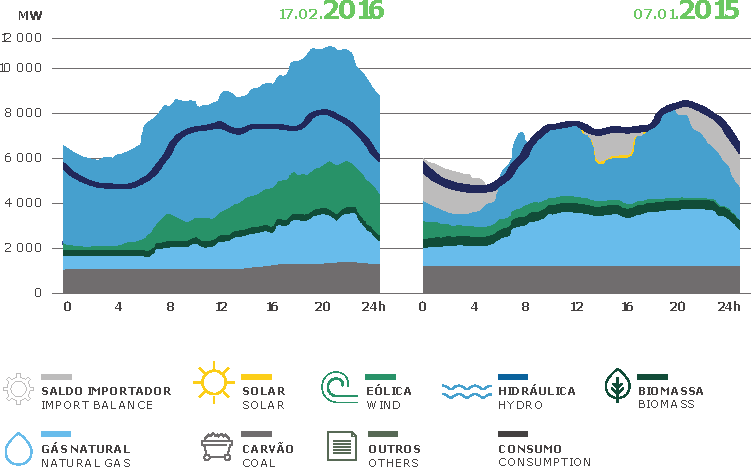
\includegraphics[width=0.7\linewidth]{img/ConsumoDiaDePontaAnual.pdf}
	\caption{Diagrama de Consumo no Dia de Ponta Anual}
	\vspace{-3.5mm}
	\caption*{Fonte: \citeonline{REN}}
	\label{fig:ConsumoDiaDePontaAnual}
\end{figure}

Em 2016 houve um total de  1130 horas em que a eletricidade renovável por si só, foi suficiente para suprir as necessidades elétricas de Portugal. Ainda neste ano, entre as 6:45h do dia 7 e 17:45h do dia 11 de maio, foi registrado um período de 107 horas consecutivas em que a produção renovável excedeu o consumo elétrico \cite{apren}. Estes fato que demonstra que mesmo com o aumento do consumo, a geração renovável e supera o consumo em vários períodos relevantes. 

Segundo a \citeonline{apren} em 2016 houve um importante marco do saldo exportador de 5,1 TWh, que constitui uma inversão na tendência de importação apresentada nos últimos 15 anos. O gráfico da Figura \ref{fig:SatisfacaoDoConsumo} trás um comparativo da satisfação do consumo anual entre 2007 e 2016. 

\vspace{5.5mm}

\begin{figure}[H]
	\centering
	\captionsetup{width=0.7\textwidth, font=footnotesize, textfont=bf}	
	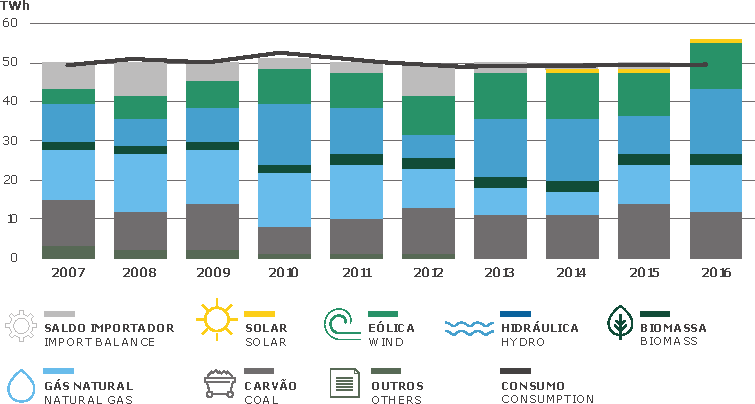
\includegraphics[width=0.7\linewidth]{img/SatisfacaoDoConsumo.pdf}
	\caption{Satisfação do Consumo}
	\vspace{-3.5mm}
	\caption*{Fonte: \citeonline[p.~10]{REN}}
	\label{fig:SatisfacaoDoConsumo}
\end{figure}